\section{Image binarization}

The inbuilt Matlab function \textit{imbinarize} creates a logical array for an grayscale image I given a threshold t in which all pixels with values above t get mapped to a 1 and all other pixels to a 0.

Figure \ref{fig:task19} shows binarizations for a grayscale image of a car for different thresholds. It can be seen that it depends heavily on the specific image which threshold results in a useful binarization. In this case, a threshold of 20 or 30 still maps most pixel to white pixels and does not yield a useful result. When moving the threshold closer to 1, most pixels get mapped to a black output, as the in the last image of figure \ref{fig:task19}.

\begin{figure}[!hbt]
  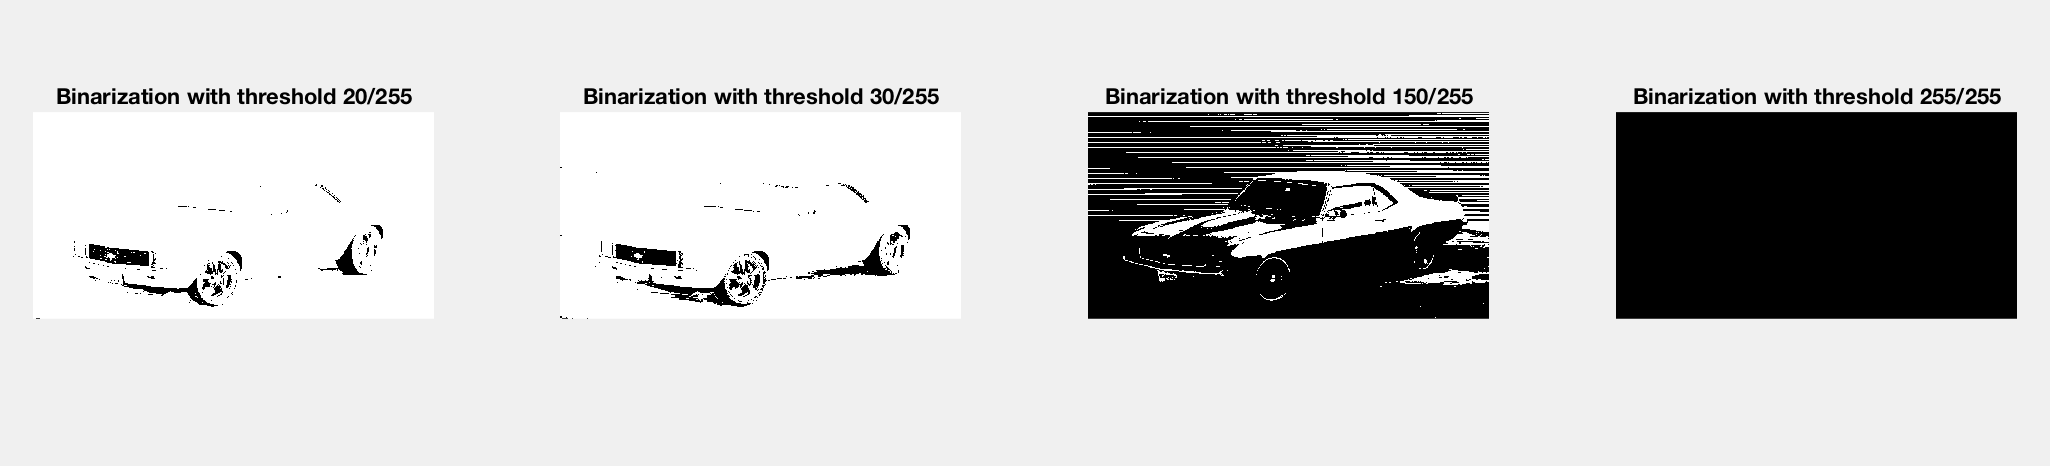
\includegraphics[width=\textwidth]{./img/task19.png}
  \caption{Image binarization with different thresholds}
  \label{fig:task19}
\end{figure}

Figure \ref{fig:task20} shows the pixel-wise product of the original image and its binarization with a threshold of 150/250.

\begin{figure}[!hbt]
  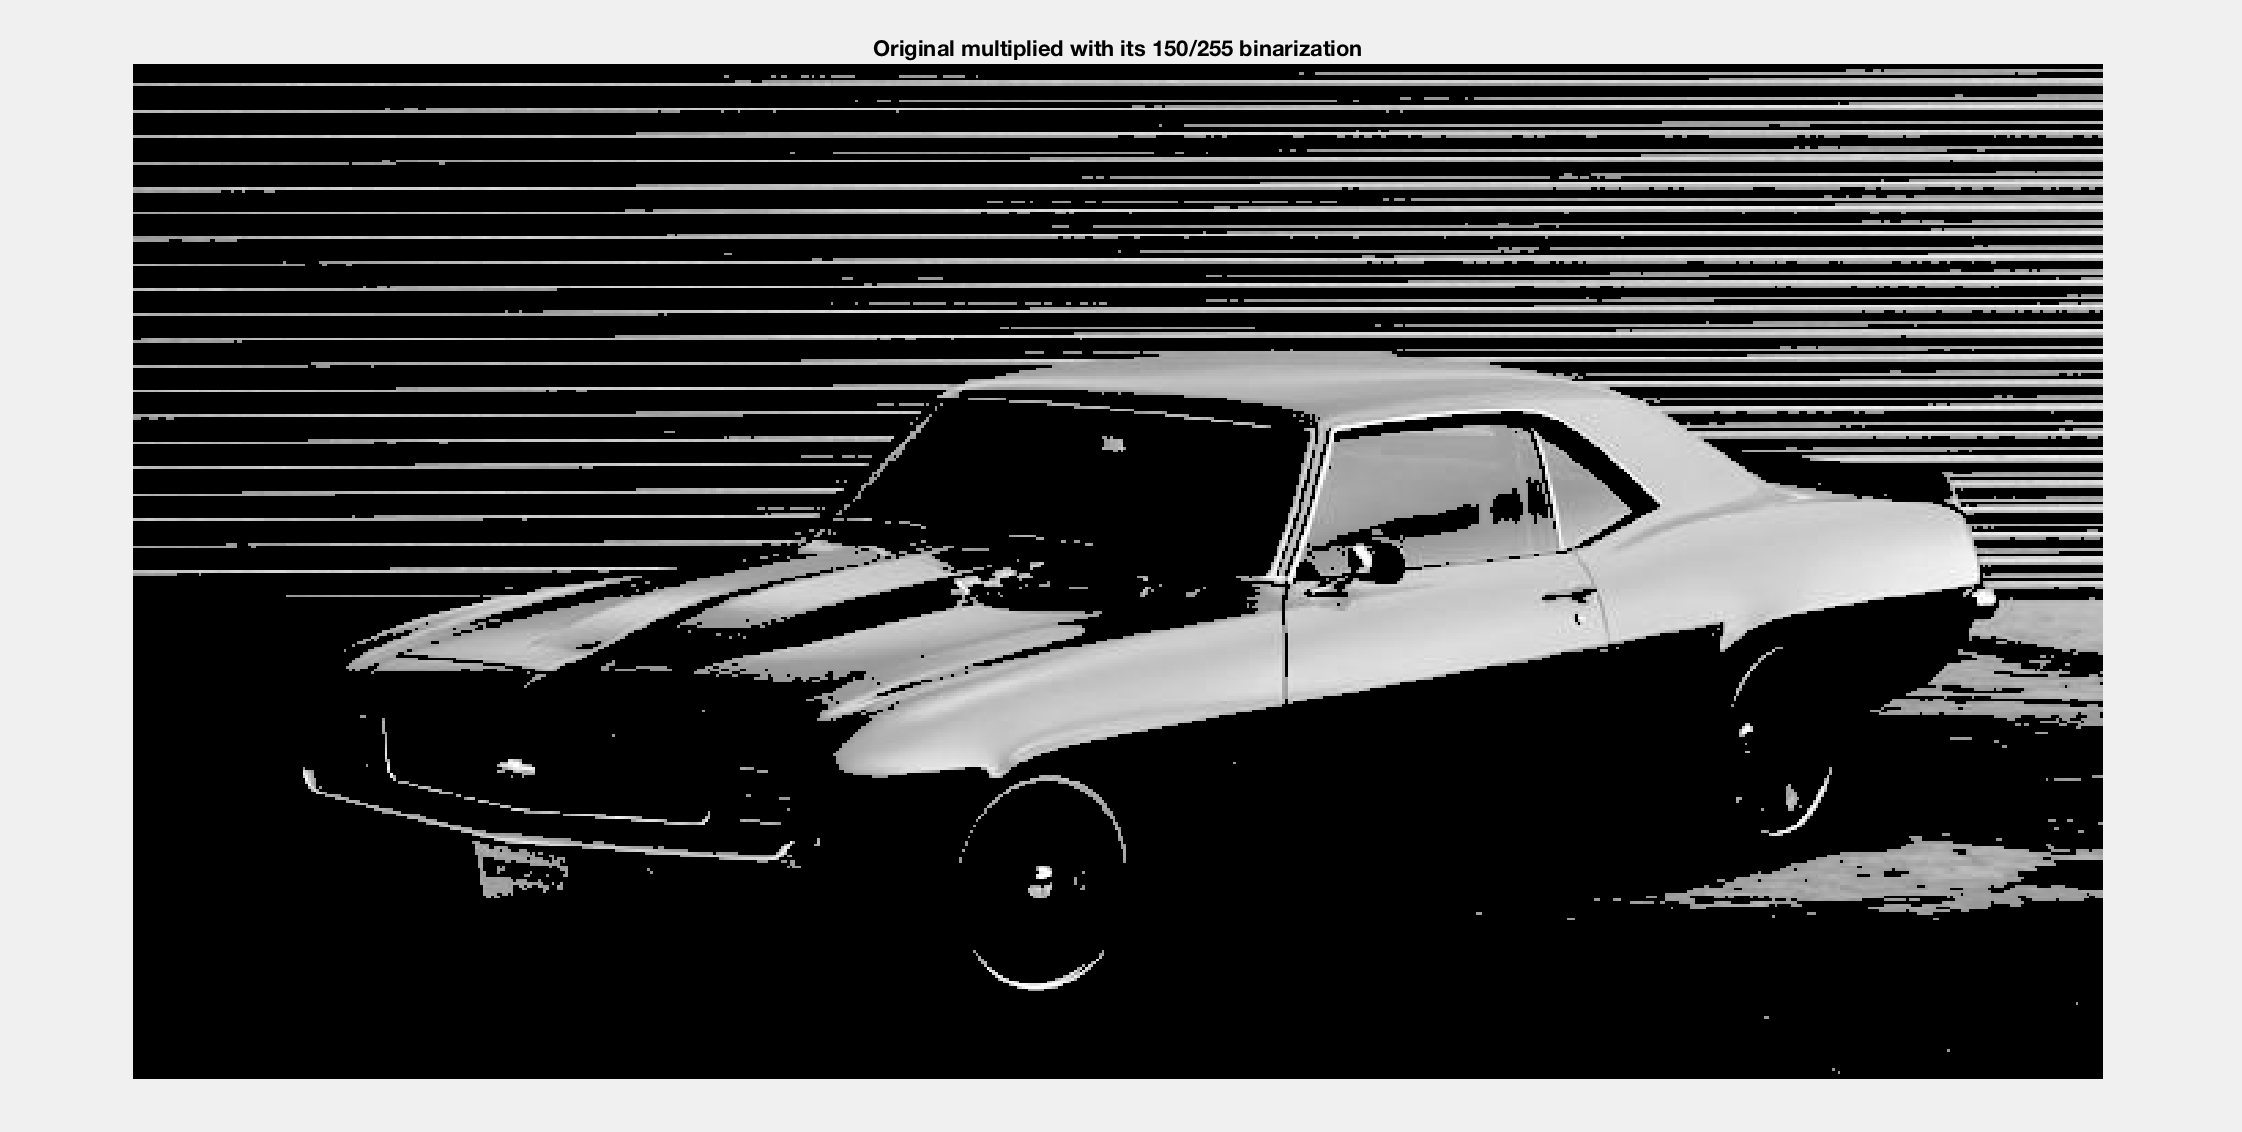
\includegraphics[width=\textwidth]{./img/task20.png}
  \caption{Original multiplied with its binarization}
  \label{fig:task20}
\end{figure}

Figure \ref{fig:task21} shows the pixel-wise product of the original image and its inverted binarization with a threshold of 150/250.

\begin{figure}[!hbt]
  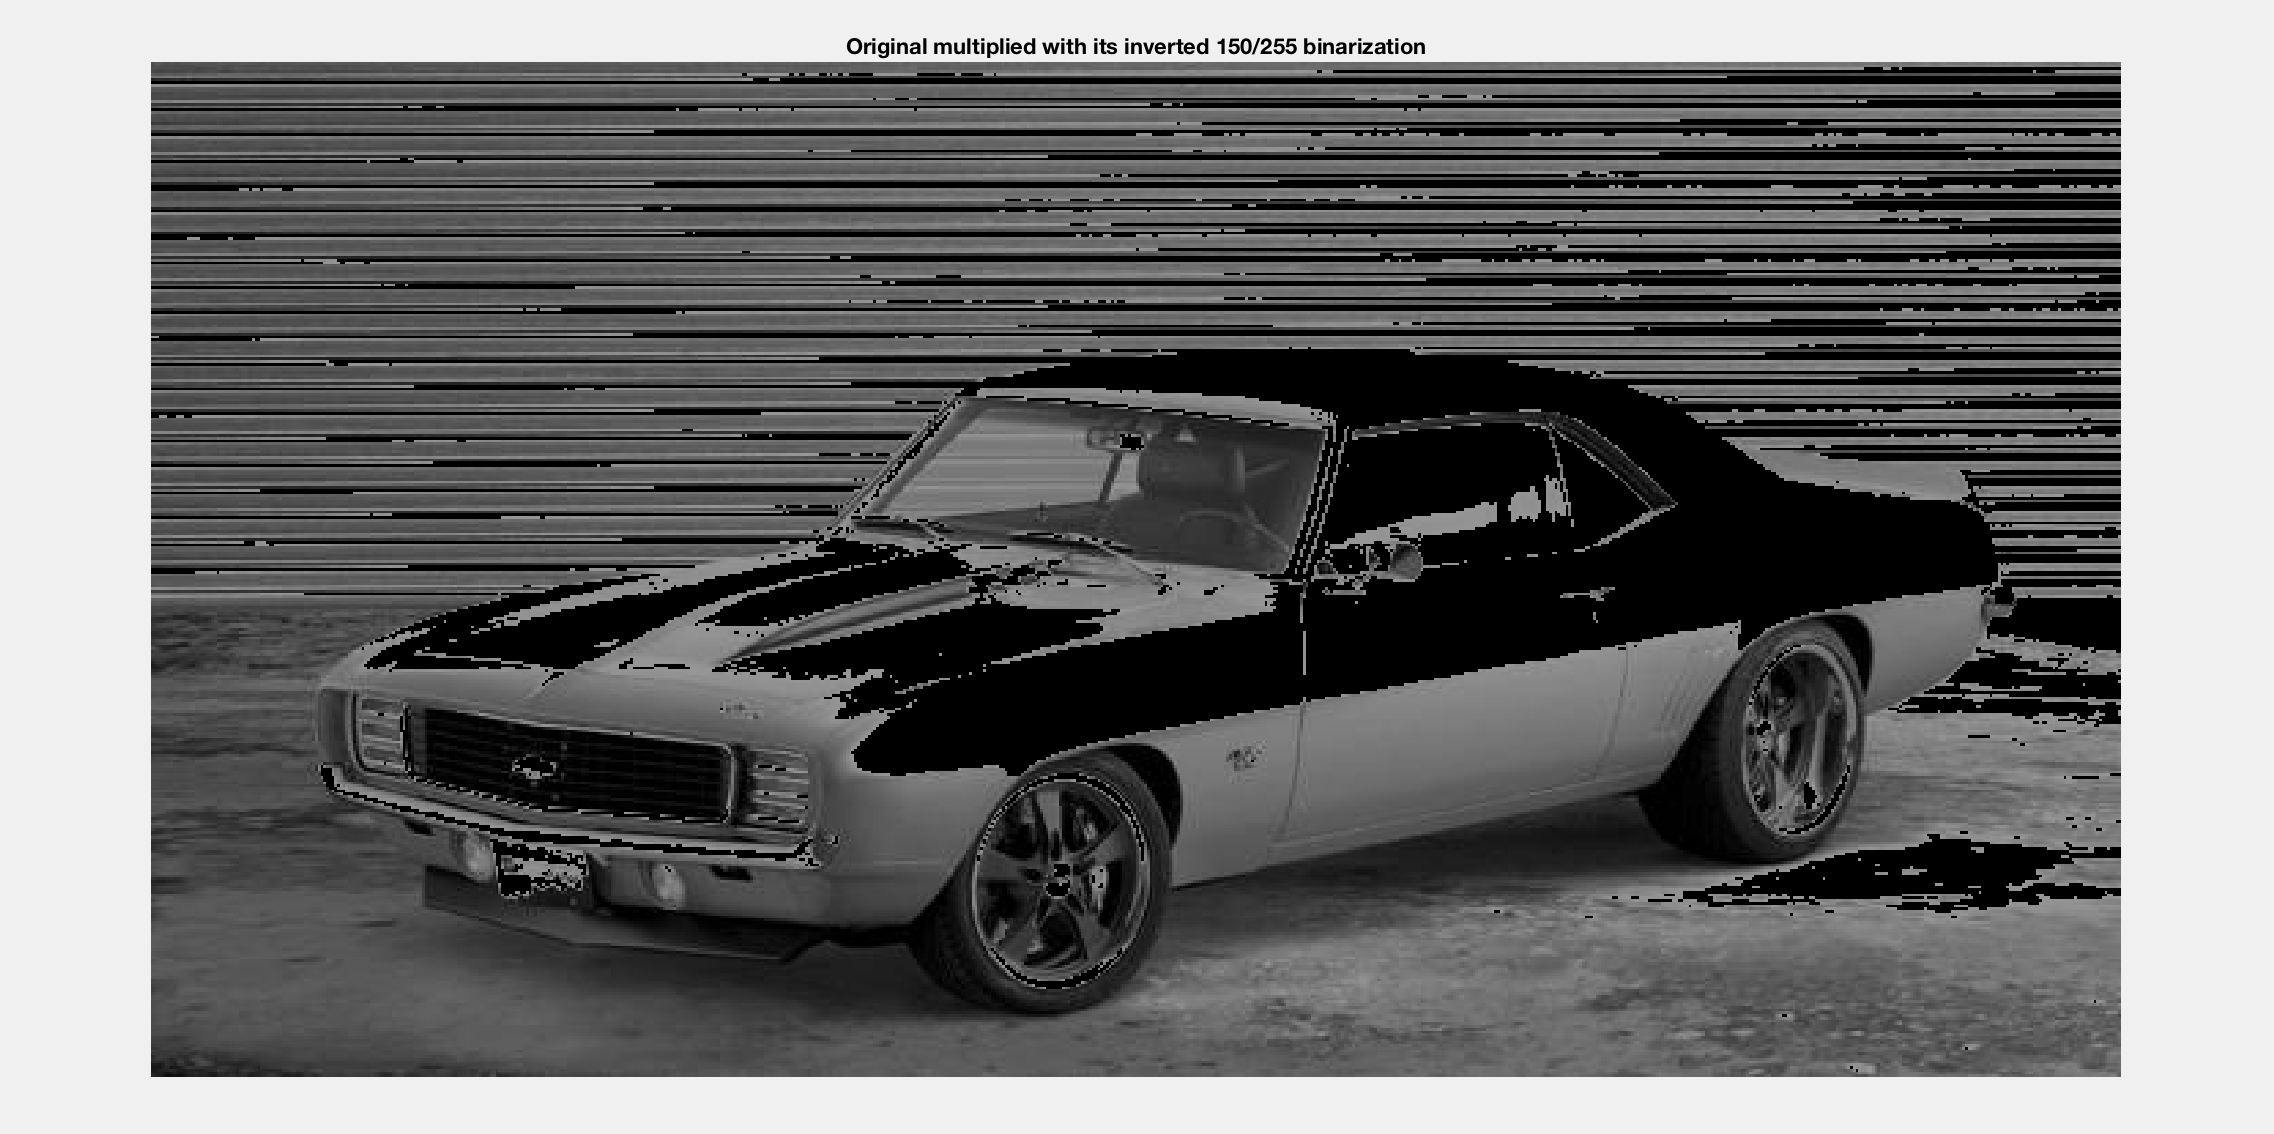
\includegraphics[width=\textwidth]{./img/task21.png}
  \caption{Original multiplied with its inverted binarization}
  \label{fig:task21}
\end{figure}